\section{Профилирование}

Профилирование проводилось с помощью утилиты \verb|perf|.

\linespace

Профилировалась утилита \verb|ps-scanner|. Была собрана информация о (\%) загруженности CPU, функциях программ в пользовательском пространстве и функциях ядра.\\
С помощью \verb|perf record| была собрана данная статистика и сохранена в директории \verb|./profiling/perf.data|, в данном случае профилировались все процессы (\verb|-a|), а также собиралась трассировка стека (\verb|-g|).

\linespace

Далее с помощью \verb|perf script| была выведена информация в виде текста, которые собрала \verb|perf|. Полученные данные можно анализировать скриптом. Например Flamegraph-скриптом.

\linespace

Flamegraph -- это отличный способ визуализировать профилированные данные. На данном графе можно посмотреть сколько трассировок приходится на функции. Для более подробного просмотра можно воспользоваться браузером:
\begin{lstlisting}[language=bash]
$ firefox ./profiling/perf.svg
\end{lstlisting}

\newpage

\begin{center}
    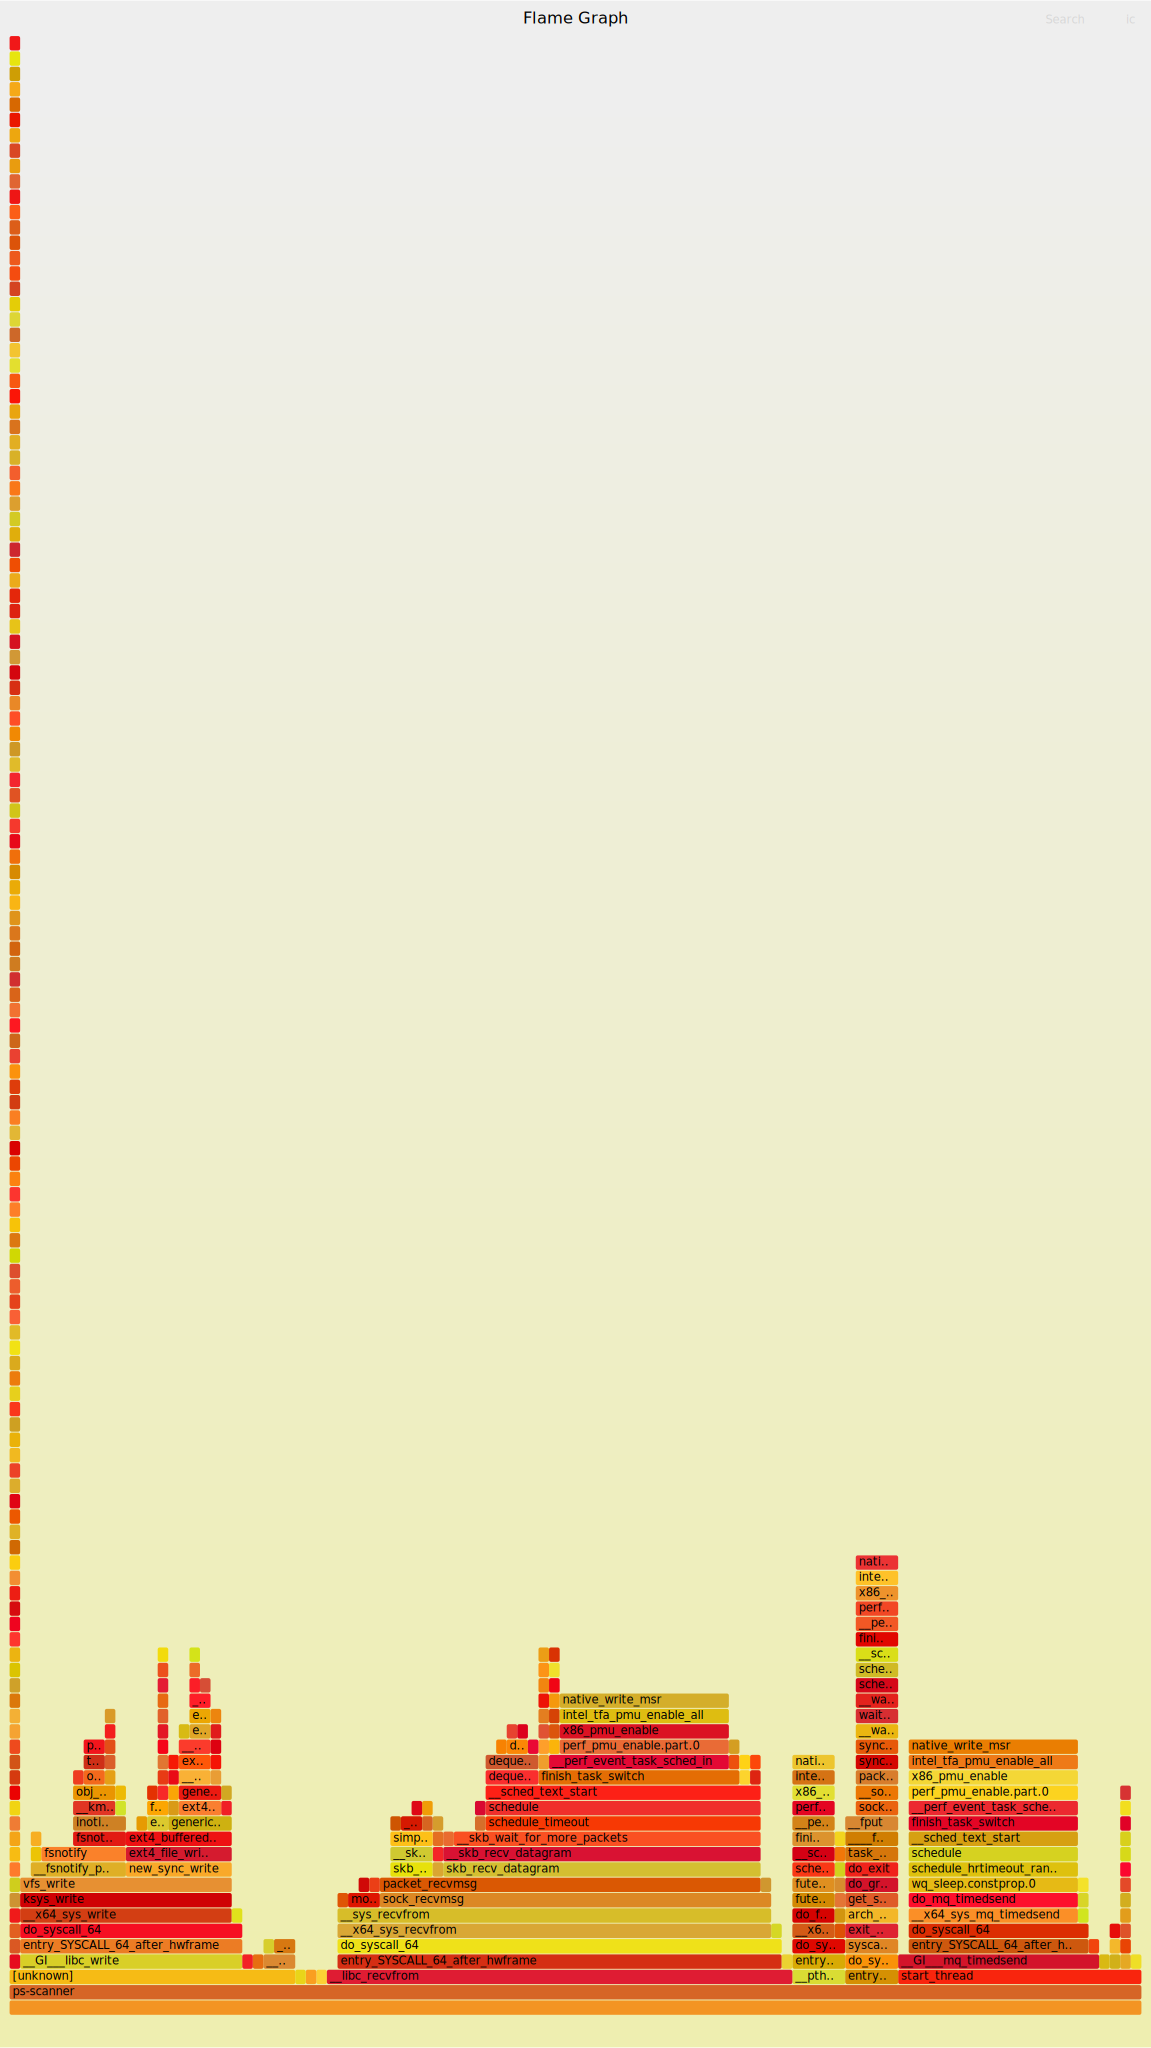
\includegraphics[scale=0.34]{../assets/perf.png}
\end{center}
